% =====================================================================
%  Chapter 17 — A Panel Regression as a Conjugate Update
% =====================================================================

\chapter{A Panel Regression as a Conjugate Update}
\label{ch:conjugate}

The book's model is a linear regression on a panel of funds, with a prior
that happens to be conjugate to the likelihood. This chapter derives it,
explains why a prior is not optional, and shows how the same equations
produce both the forecast and --- more importantly --- the uncertainty in
the forecast.

\section{Why a prior is not optional}

Consider the regression a reader might expect: fit a linear model of the
future return on twelve features, using all the data, and use the fitted
coefficients as the forecast.

That procedure has no way to express uncertainty, and it has a second
problem that is harder to see. The number of coefficients is twelve. The
number of observations in the training set is the number of months times
the number of funds, which in the early years is small and in the later
years is large. When the second is not much larger than the first, the
least-squares estimate of each coefficient is enormously unstable --- the
variance of the estimate is proportional to the inverse of the
information matrix, and an ill-conditioned information matrix produces
coefficients that are large and individually meaningless.

A prior fixes this. It is a statement about how much the data should be
allowed to move the coefficients, expressed as a precision. The book's
model puts a prior precision of \(0.5\) or \(2.0\) on each coefficient
around a prior mean of zero, and the two values appear in the trial family
precisely because the strength of the prior is a parameter that changes
what the model is willing to believe.

\section{The model}

For fund \(i\) at formation date \(t\), with feature vector \(x_i \in
\mathbb{R}^{k}\) (standardised, and with a constant of one appended so
that the model has an intercept), the model is

\begin{equation}
y_i = x_i^{\prime}\beta + \varepsilon_i,
\qquad
\varepsilon_i \sim N(0, \sigma^2),
\end{equation}
with the conjugate prior

\begin{equation}
\beta \mid \sigma^2 \sim N(m_0,\ \sigma^2\Lambda^{-1}),
\qquad
\sigma^2 \sim \mathrm{Inv\text{-}Gamma}(\alpha_0,\beta_0),
\end{equation}
where \(\Lambda = \lambda I_k\) is the prior precision and
\(\alpha_0 = 2.5\), \(\beta_0 = 0.5\) throughout.

The parameter \(\lambda\) deserves a sentence, because it is the one place
where a reader might reasonably object that a prior has been imposed where
the data should speak. A precision of \(0.5\) on a standardised
coefficient is a weak prior: it says that before seeing any data, a
coefficient is probably within about \(\sqrt{1/0.5} = 1.4\) standard
deviations of zero. A precision of \(2.0\) is stronger. Neither is
enough to prevent the data from speaking, and both are enough to prevent
a single lucky month from producing a coefficient of eight.

\section{The posterior}

Because the prior is conjugate, the posterior is available in closed form
and the update is a matrix identity. With \(n\) training observations,
design matrix \(X\), and response vector \(y$, the posterior precision and
mean are

\begin{equation}
A_n = X^{\prime}X + \Lambda,
\qquad
A_n^{-1} = \Lambda^{-1} + (X^{\prime}X)^{-1},
\end{equation}
\begin{equation}
m_n = A_n^{-1}\left(X^{\prime}y + \Lambda m_0\right).
\end{equation}

The scalar parameters update in the same step:

\begin{equation}
\alpha_n = \alpha_0 + \frac{n}{2},
\qquad
\beta_n = \beta_0 + \frac{1}{2}
  \left(y^{\prime}y + m_0^{\prime}\Lambda m_0 - m_n^{\prime}A_n m_n\right).
\end{equation}

Note what is happening. The posterior mean \(m_n\) is the prior mean
weighted by the prior precision plus the data weighted by the data
precision, combined through the joint precision \(A_n\). It is the
weighted average of what was believed and what was observed, with weights
that depend on how much each is worth. When the data is abundant relative
to the prior, the data dominates; when it is scarce --- and in the early
years of this book it is --- the prior holds the coefficients near zero
and the model produces small forecasts with correspondingly large
uncertainties.

The residual scale is estimated as
\begin{equation}
\hat{\sigma}^2 = \frac{\beta_n}{\alpha_n - 1}.
\end{equation}

\section{The prediction, and the part that matters}

For a new observation with features \(x_*\), the posterior predictive
mean is

\begin{equation}
\mu_* = x_*^{\prime} m_n,
\end{equation}
and there are two variances that must not be confused.

The posterior variance of the \emph{observation} is
\begin{equation}
v_{\mathrm{obs}} = \hat{\sigma}^2\left(1 + x_*^{\prime}A_n^{-1}x_*\right),
\end{equation}
which is the variance of what the return will be, conditional on the
model being right.

The posterior variance of the \emph{mean} is
\begin{equation}
v_{\mathrm{mean}} = \hat{\sigma}^2 x_*^{\prime}A_n^{-1}x_*,
\end{equation}
which is the variance of the \emph{estimate} of the expected return. It is
the smaller of the two, and it is the one that governs how much the
investor should believe.

\begin{takeaway}[The distinction the whole book turns on]
\(v_{\mathrm{obs}}\) is the risk of the asset. \(v_{\mathrm{mean}}\) is the
doubt about the forecast. A model that reports only the first has told
the investor nothing useful; a model that reports only the second has
told the investor to ignore the risk. The portfolio layer needs both, and
Chapter 26 shows exactly where each enters.
\end{takeaway}

\section{Walk-forward estimation}

The model is refitted at every formation date \(t\), and the training set
at \(t\) contains only the rows whose target has already been realised.

If the horizon is \(h\), a row formed at date \(s\) has its outcome
realised at \(s+h\), so the training set at \(t\) is

\begin{equation}
\mathcal{D}_t = \{(x_i, y_i) : s_i + h \le t\},
\end{equation}
and the rows are taken as a prefix of the long-format design matrix, which
is why the implementation sorts the rows by date and slices.

The implementation also imposes two warm-up conditions before it will
produce a forecast at all: a minimum number of months of history, and a
minimum number of training rows relative to the number of features. Both
exist to prevent the pathological regime in which a model with twelve
coefficients is fitted to fifty observations and produces a forecast with
wildly confident wrong coefficients.

\begin{figure}[!htbp]
\centering
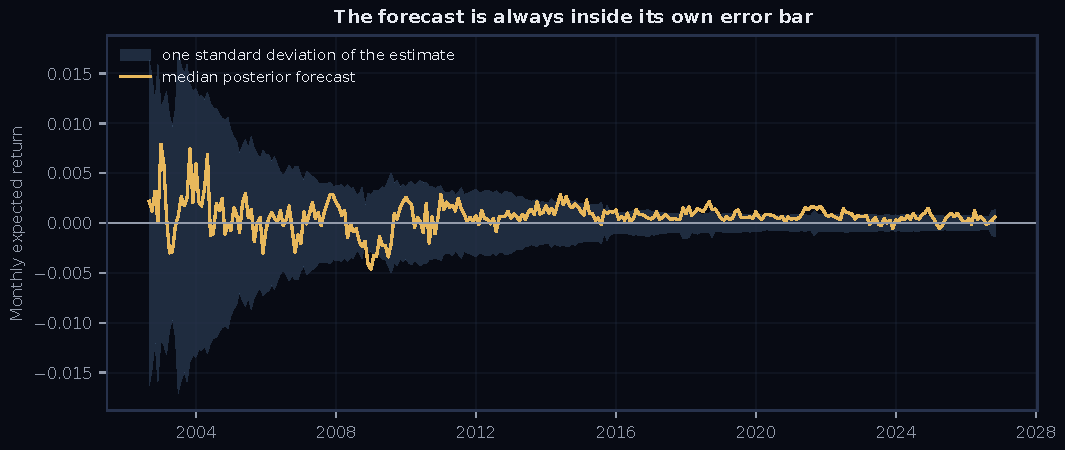
\includegraphics[width=\textwidth]{../figures/fig_posterior.pdf}
\caption{The posterior machinery in one picture. The left panel shows the
posterior mean and the posterior credible interval of the expected
one-month forward return for a representative fund over the record; the
right panel shows the ratio of the posterior variance of the mean to the
posterior variance of the observation --- the fraction of the uncertainty
that is doubt about the forecast rather than risk of the asset.}
\label{fig:posterior}
\end{figure}

\figref{fig:posterior} is the figure the whole architecture exists to
produce. The credible interval on the left is wide, and it should be: the
model is estimating a three-month expected return from price history, and
the honest answer is that it does not know it very well. The panel on the
right says something more useful still: the doubt about the forecast is a
substantial fraction of the total uncertainty, which means that sizing a
position on the forecast alone --- ignoring the doubt --- would be sizing
it as though it were known.

\begin{keytakeaways}
\item The model is a Bayesian linear panel regression with a normal
inverse-gamma prior whose strength is a stated, tested parameter.
\item The conjugate update gives the posterior mean as a precision-weighted
blend of the prior and the data, so the prior holds the coefficients near
zero exactly when the data is thin.
\item Two variances come out of the fit and they are not interchangeable:
the variance of the observation is risk, and the variance of the mean is
doubt about the forecast.
\item The model is refitted at every formation date on rows whose outcome
has already been realised, and refuses to forecast at all until the
warm-up conditions are met.
\end{keytakeaways}
